\section{Preliminary Implementation} \label{sec:implementation}

We have implemented a prototype of \sysname on a testbed of clustered bare-metal
machines (Intel Xeon 2.40GHz 4-cores CPU, 67 GB of memory, 40Gbps Mellanox CX3
NIC, CentOS 7). The prototype will select the most
efficient data-plane mechanism based on the location of two containers: 
if the two containers are intra-host, shared-memory mechanism will be selected for data
transfer, and if the two containers are inter-host, RDMA will be selected.
We implemented the shared-memory via multiplexing \texttt{IPC namespace}, and enabled
containers to use RDMA by using the \texttt{host mode}.
We evaluated our prototype and compare it with state-of-the-art container overlay network
 - \texttt{Weave}, and shown that the prototype
can achieve higher throughput, lower cpu usage and smaller latency for both intra-host
and inter-host cases. The measurement result is presented in Figure~\ref{fig:sys_eval_proto}

     \begin{figure}[ht]
     \centering 
     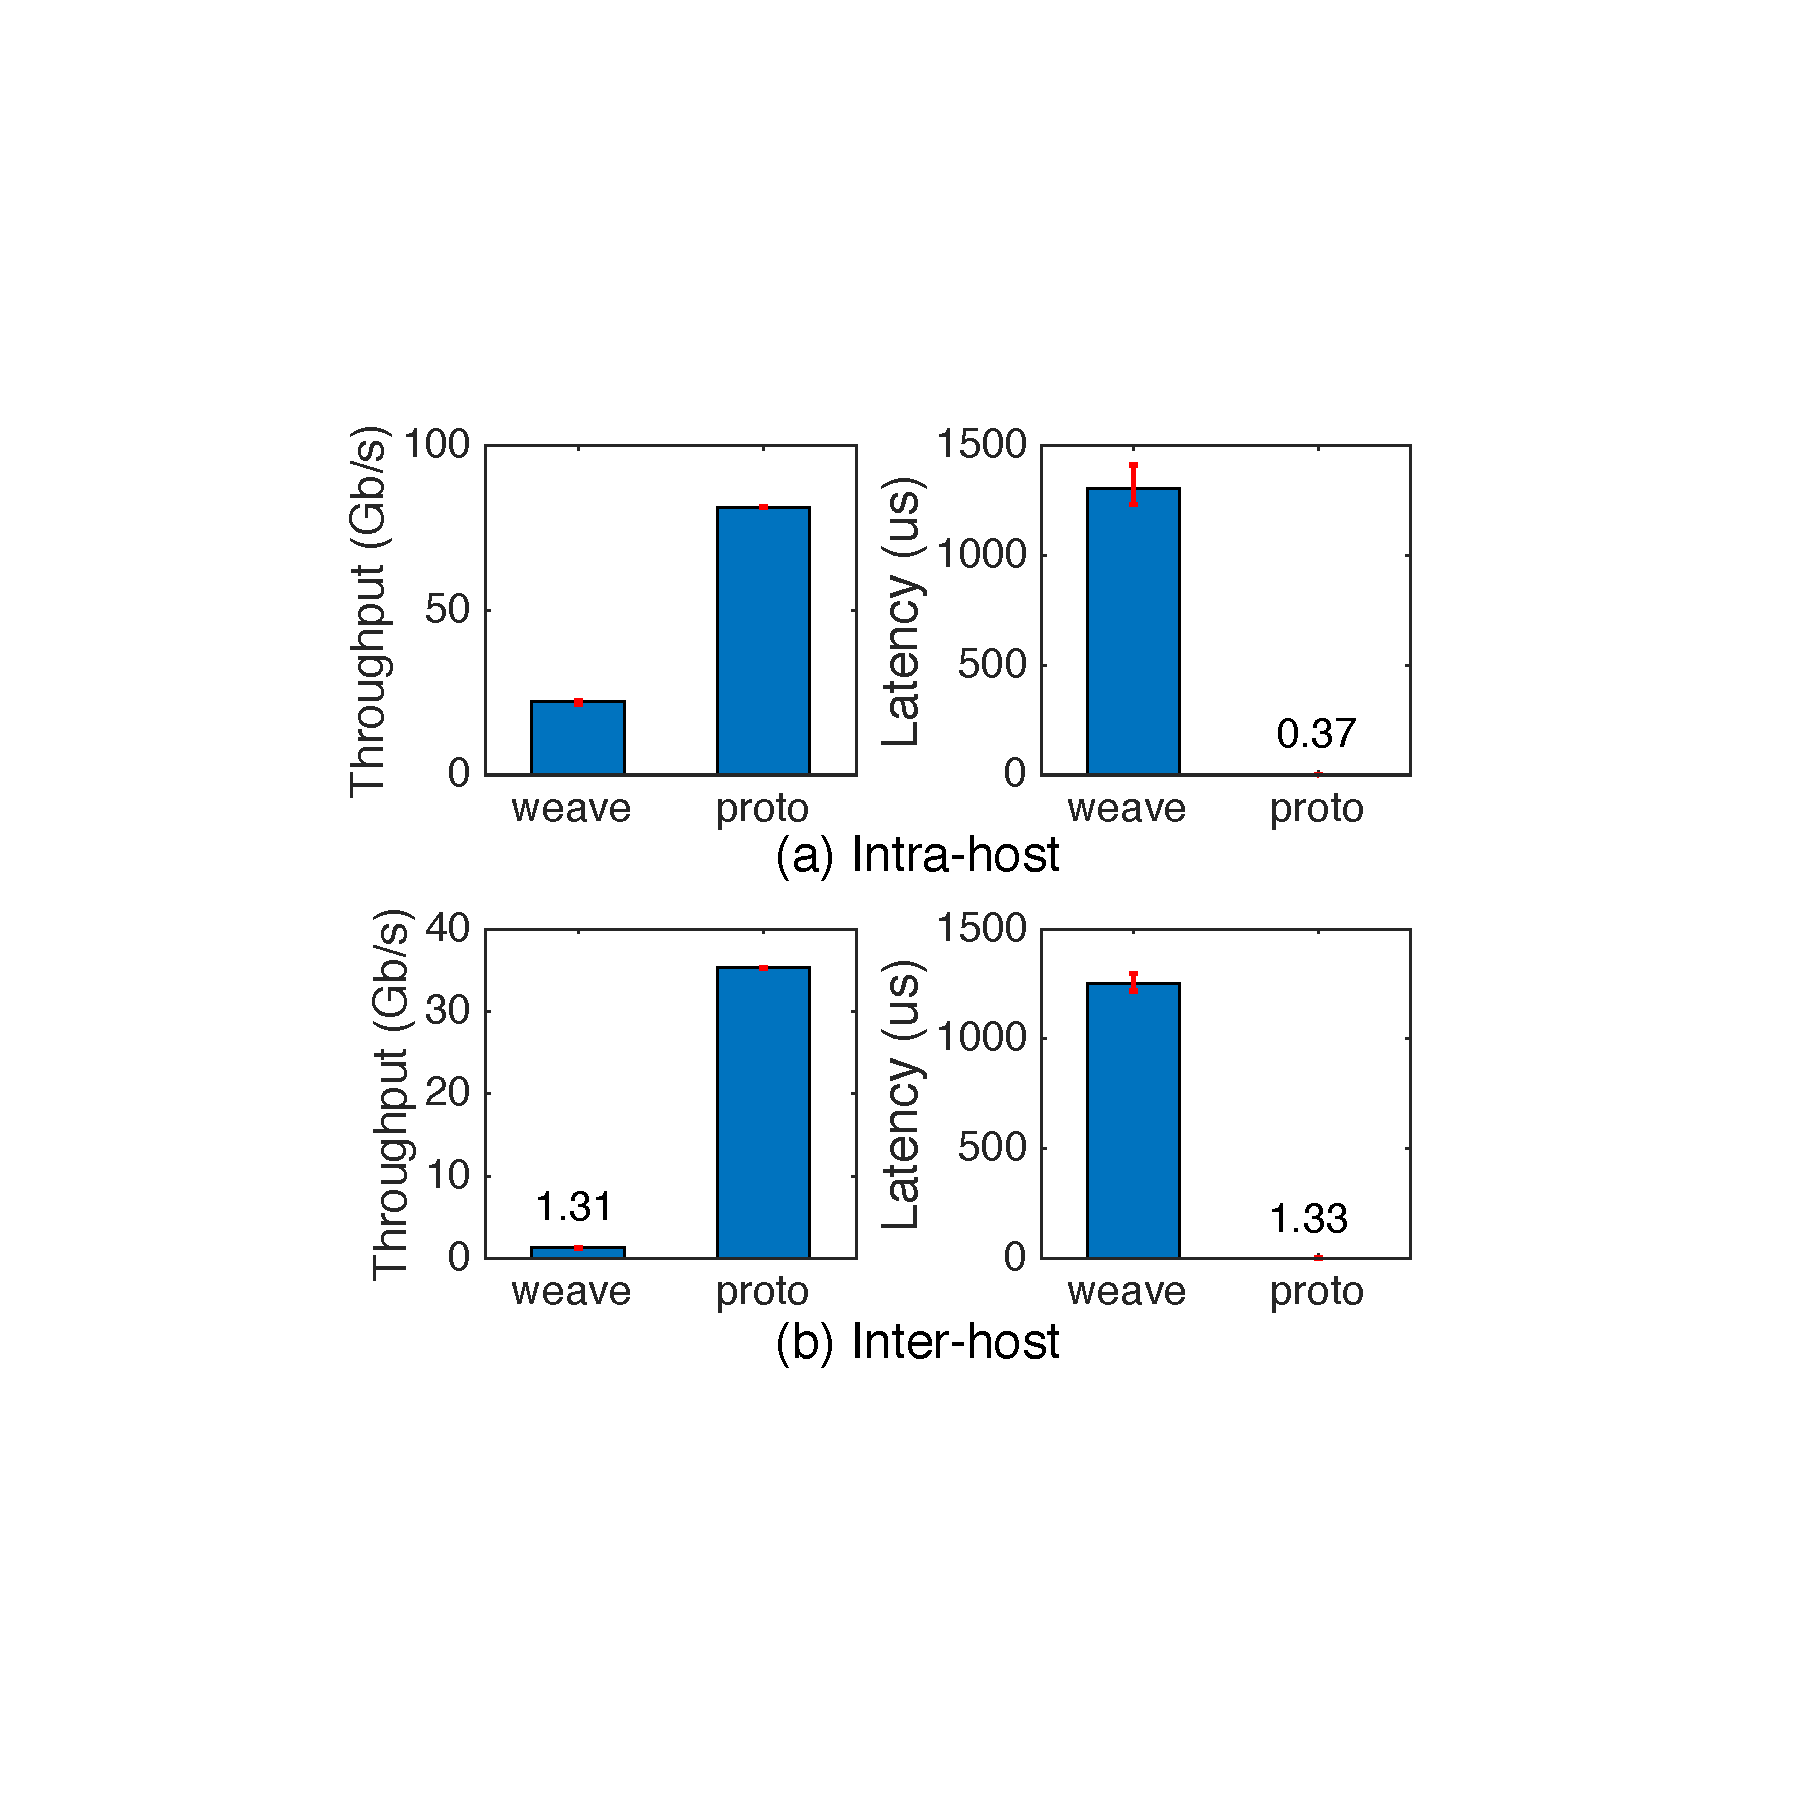
\includegraphics[width=0.45\textwidth]{figures/system/eval_proto.pdf}
     \label{fig:sys_eval_proto}
     \caption{Compare \sysname prototype with weave.} 
     \end{figure}


%%% commented 
\iffalse

In this section, we show our roadmap to realize \sysname and a preliminary 
implementation.

\subsection{Network orchestrator}

The main functionality of the network orchastrator is to feed network agents
the realtime information of container locations and VM locations (if needed).
Since containers are typically started and managed by a cluster orchestrator
(e.g. Marathon/Mesos), the container to host mapping can be easily accessed
from the cluster orchestrator. \sysname only adds a small module into 
existing clusters orchstrators to push the newest container-to-host mapping
to all network agents in the cluster. Similary, if hosts are VMs and further optimizations are needed for the communications in case (c) and (d) in 
Figure~\ref{fig:deploycases}, \sysname adds a similar module to cloud fabric
controllers (e.g. OpenStack Nova) to push the newest VM-to-machine mapping
to network agents.

\subsection{Network agent}

     \begin{figure}[t!]
     \centering 
     \begin{subfigure}
     \centering 
     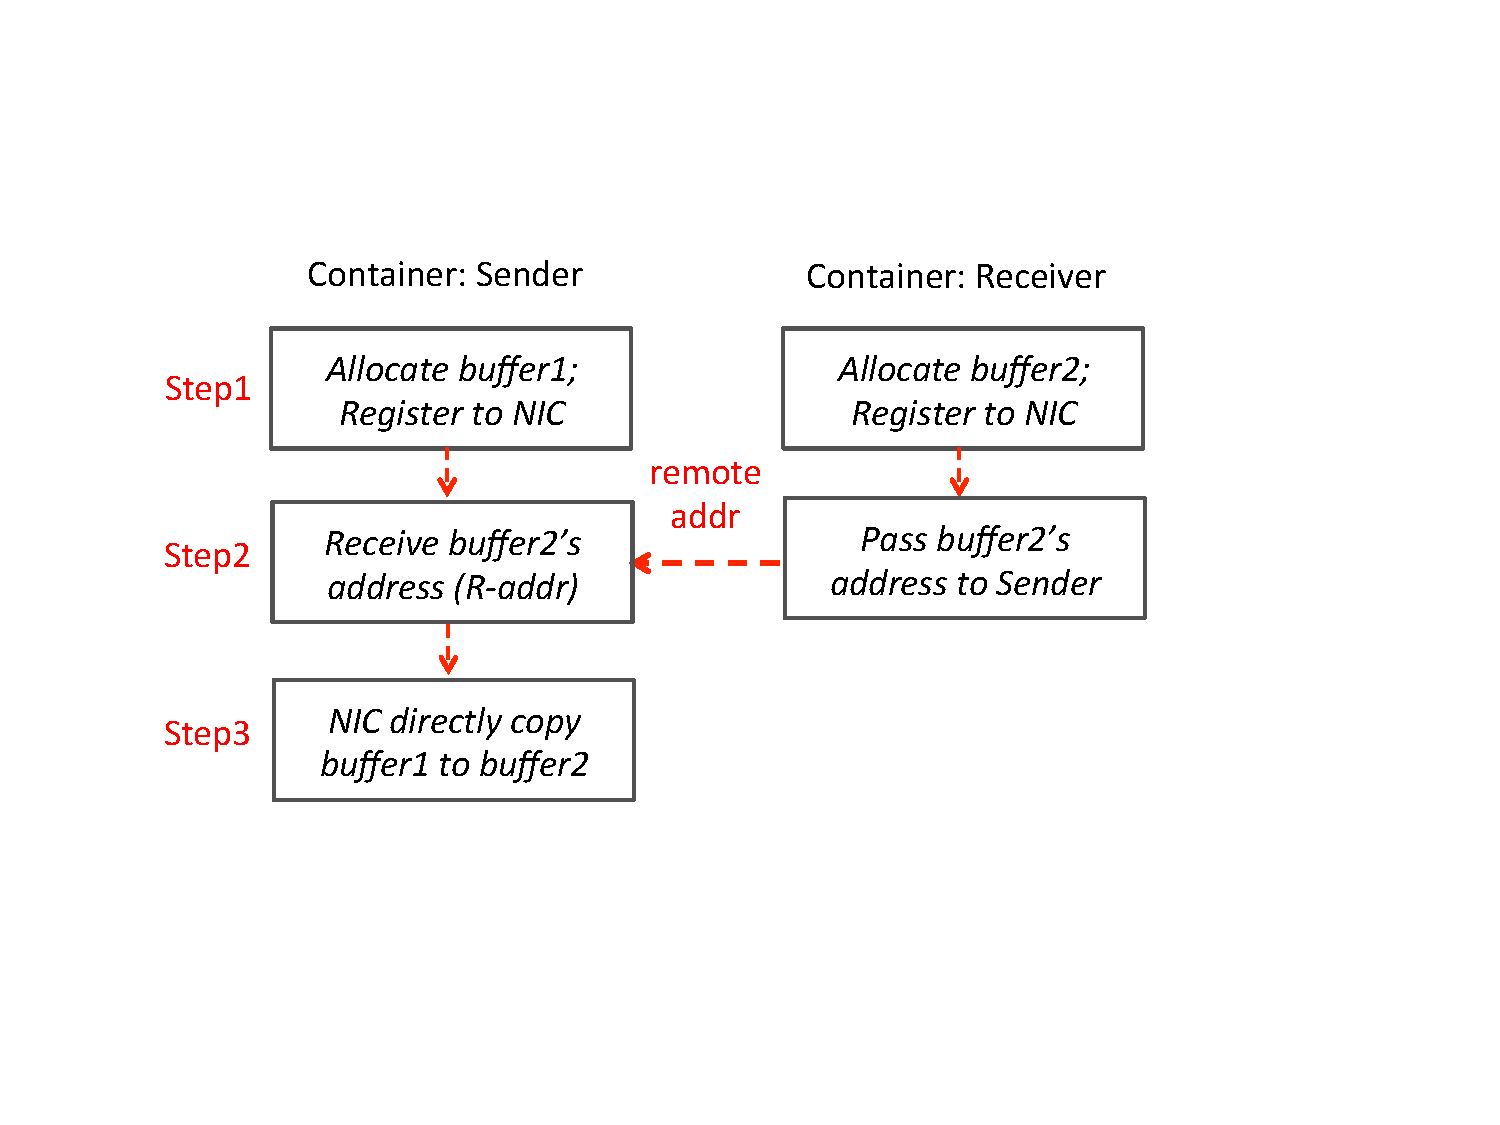
\includegraphics[width=0.45\textwidth]{figures/system/sys_rdma_steps.pdf}
     %\caption{\label{fig:fig1}}
     %\caption{steps} 
     \end{subfigure}
           
     \begin{subfigure}
     \centering 
     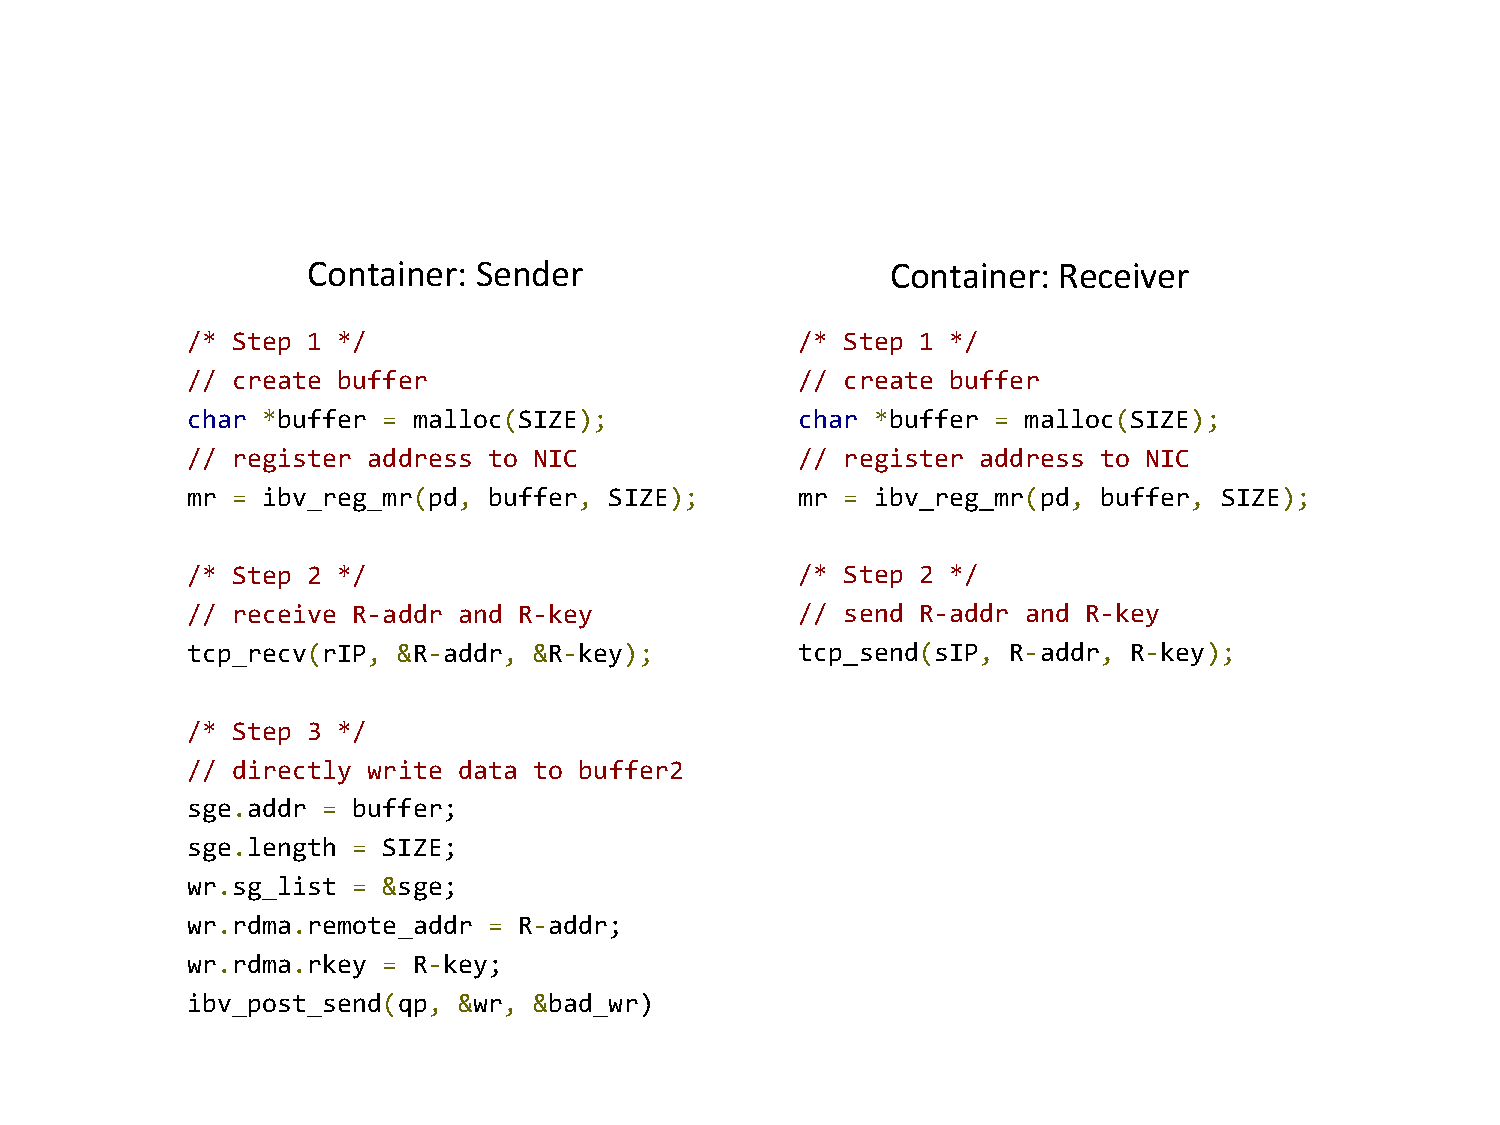
\includegraphics[width=0.45\textwidth]{figures/system/sys_rdma_code.pdf}      
     %\caption{\label{fig:fig2}}
     \end{subfigure}
     \label{fig:sys_rdma_steps_code}
     \caption{The steps and pseudo code of applications executing a RDMA Write.} 
     \end{figure}

Network agent decides which data-plane mechanism to use for data transfers
between containers. Because the network abstrction layer has already convert
data transfers uniformly to standard RDMA operations, network agent can simply
handle RDMA Write and Read operations between containers (or actually vNICs
of containers). We take Write as an example to explain the working flow of
network agent, and Read will be similar.

Conceptually, network agent needs to enable two containers to use shared-memory
to communicate if they are in the same host (so managed by a single network
agent). Otherwise, it tries to create a real RDMA channel to delivery the data.
However, no matter which choice it makes, the vNIC of a container should always
feel like that it is writing data directly to another vNIC with standard RDMA.

\para{Standard RDMA Write} First, standing at a vNIC's point of view, we show
the process of a RDMA write operation. 
Figure~\ref{fig:sys_rdma_steps_code} shows the three main steps with a piece of sample sample code:
\begin{itemize}
  \item Step 1: the sender create a buffer for send data (buffer1), and the receiver create a buffer for receive data (buffer2). 
Both sender and receiver register the address of the buffer with its NIC;
  \item Step 2: the receiver pass the address of buffer2 to the sender (stored in R-addr);
  \item Step 3: the sender will post the send request to the NIC along with the address of buffer1 and buffer2. The sender's
  and receiver's NIC will directly copy the data in buffer1 to buffer2.
\end{itemize}

In \sysname, the buffers created by both sender and receiver are shared
with network agent, and latter can directly manipulate the former.

\para{Intra-host case} At Step 3, the network agent directly copy the content
from buffer1 to buffer2, and notify the vNIC of the receiver when the copy is
finished. 
%Note that the memory copy from buffer1 to buffer2 is unavoidable
%because buffer1 (buffer2) will be reused or deleted by the sender (receiver).

     \begin{figure}[ht]
     \centering 
     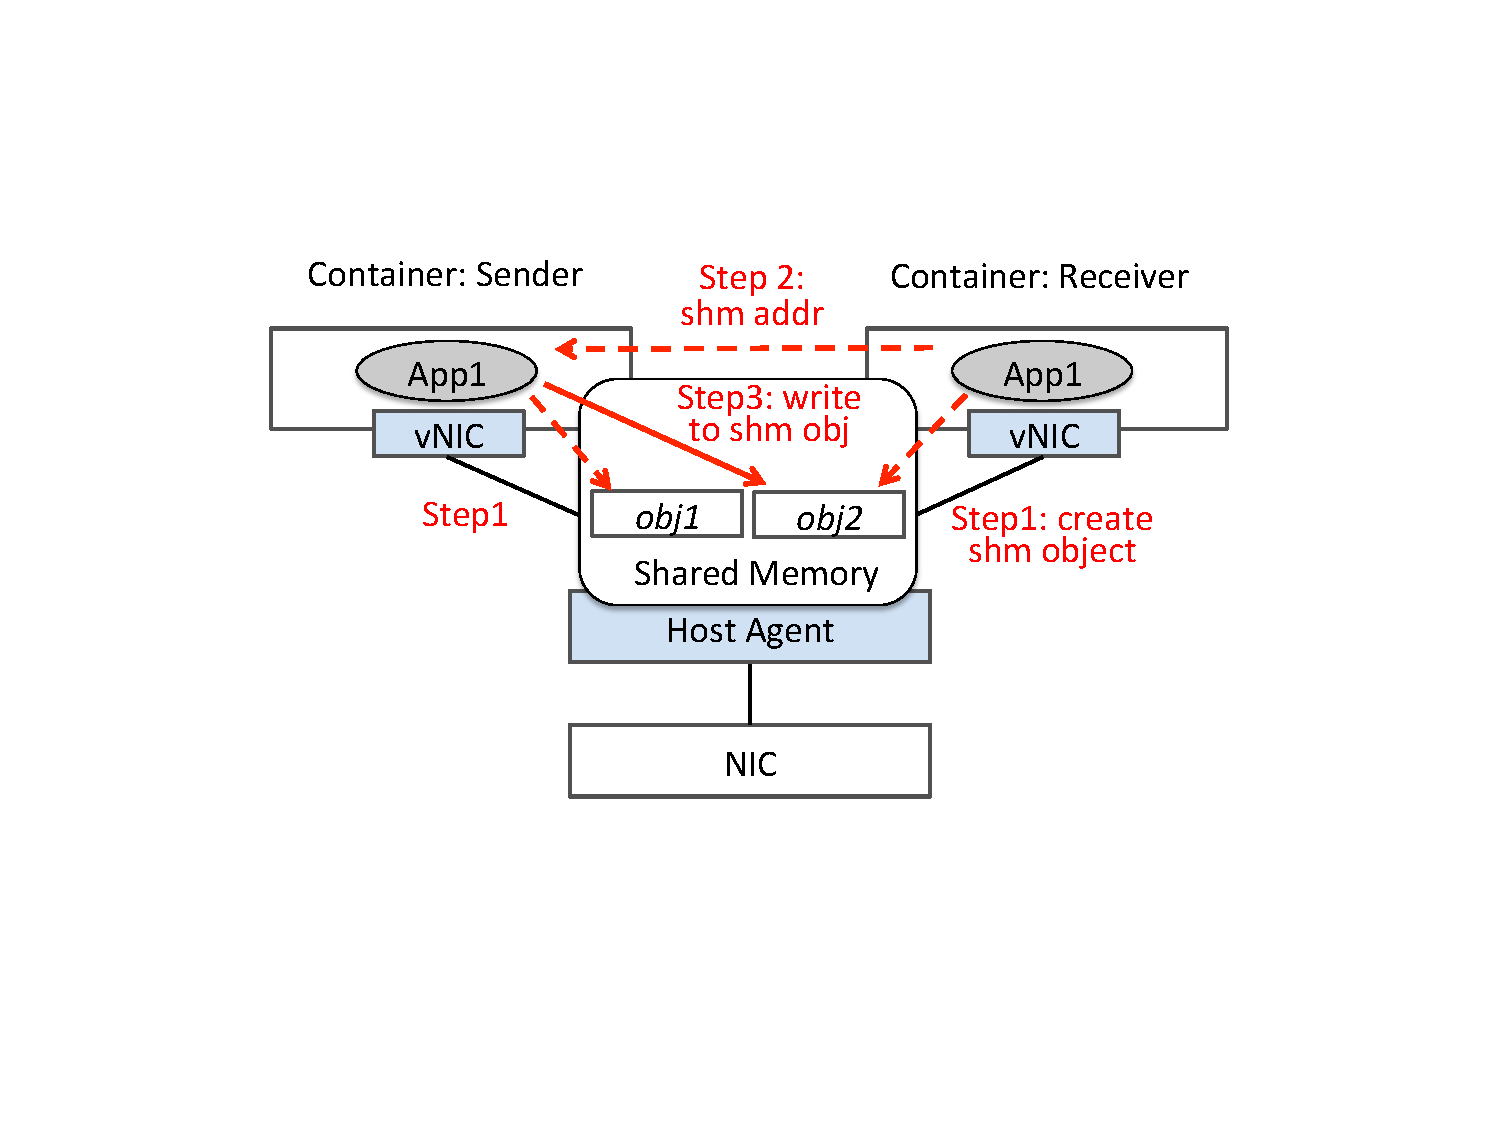
\includegraphics[width=0.45\textwidth]{figures/system/sys_rdma_shm.pdf}      
     \label{fig:sys_rdma_shm}
     \caption{How \sysname implemented RDMA write in inter-host setting.} 
     \end{figure}


\para{Inter-host case} At Step 3, the sender's network agent initiates a
new RDMA write to the receiver's network agent. In this new Write, 
both of the network agents will directly use buffer1 and buffer2, so that
the content in buffer1 will be directly copied into buffer2 via
the physical NICs. After this Write is done, the receiver's network agent
will notify the vNIC of the receiver. 

     \begin{figure}[th]
     \centering 
     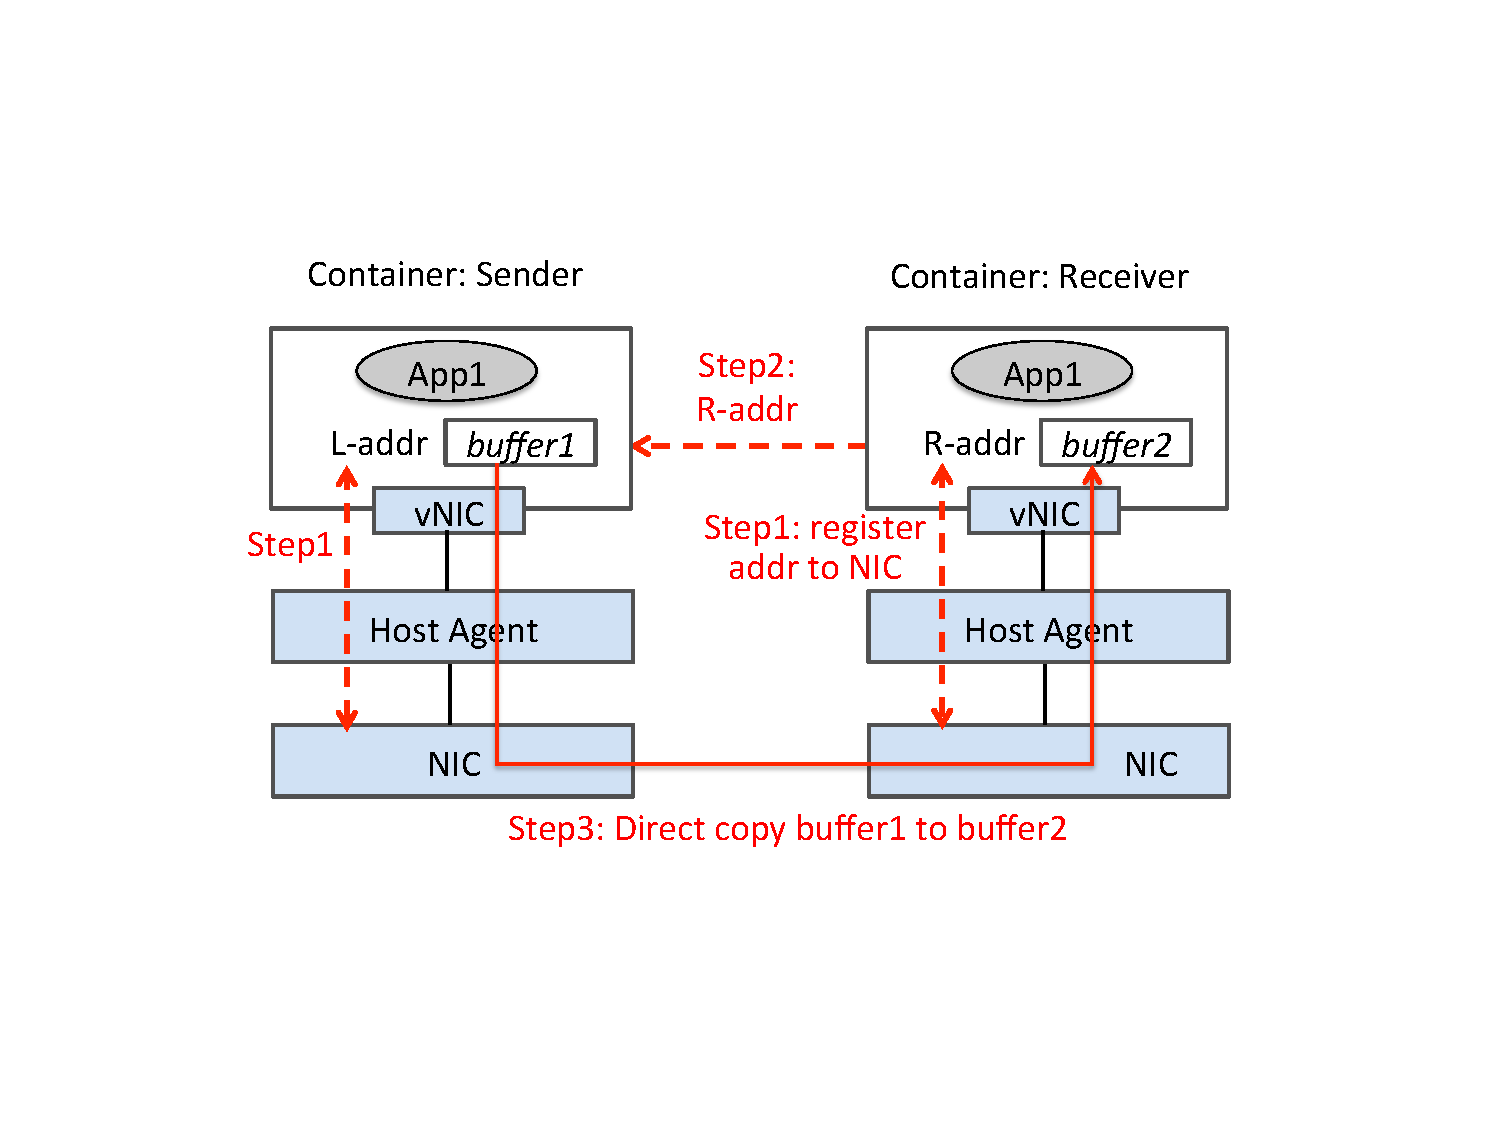
\includegraphics[width=0.45\textwidth]{figures/system/sys_rdma_rdma.pdf}
     \label{fig:sys_rdma_rdma}
     \caption{How \sysname implemented RDMA write in inter-host setting.} 
     \end{figure}


\subsection{Network abstraction}
The network abstraction layer includes vNIC, RDMA Verbs library and adaptation
libraries which translates other API calls into RDMA API calls. 
While the last two are available and we do not need to make any changes to them,
we need to develop vNIC which is a virtual NIC that understand the protocols
between RDMA programs and RDMA NICs. It forwards Write and Read requests to 
network agent and notifies the programs when a Write or Read request is finished
by network agent. 


\para{Real RDMA in inter-host setting:} First we show 
how \sysname implemented RDMA Write in inter-host setting
as shown in Figure~\ref{fig:sys_rdma_rdma}. 
In \sysname, both the sender and receiver containers have a virtual NIC (vNIC).
Different from standard RDMA Write, the applications in the container post
the send request to the virtualized network structures (e.g., RDMA Send Queue)
in the vNIC, rather than the real NIC.
The vNIC has the smartness to find out the best dataplane mechanism (by query
Mesos or Fabric Controller).
For example, in inter-host setting, RDMA is probably the best mechanism. Then
the vNIC will pass down the send request to the real NIC for RDMA transfer.


\para{Shared memory in intra-host setting:} Figure~\ref{fig:sys_rdma_shm} shows 
how \sysname implemented RDMA Write in inter-host setting.
Suppose the vNIC can find out the best dataplane mechanism for inter-host setting
is shared-memory, for example, ask the local network agent to check whether the 
receiver is on the same host of the sender.
 In step 1, both sender and receiver will create a shared memory object (equal 
to buffer in inter-host setting). The shared memory objects are inside the namespace
shared among containers and the host agent on the same physical machine.
In step 2, the receiver will pass the address of shared memory obj2 to the sender.
Then in step 3, the sender can directly write to the shared memory obj2 of the
receiver, and notify the receiver when the write is finished.



\vyas{really lost in this section. it needs a lot more structure and handholding to convince 
 me that you really have thought things through.  as it stands it sounds like  you have tried 
to talk about two narrow/corner cases but that doesnt give me any confidence that you have a solution 
sketch!}

To support the standard RDMA Verbs API used by containers and realize
communications with the best available data-plane mechanism, \sysname needs
to present a RDMA environment to containers and efficiently supports 
the RDMA semantics with multiple data-plane mechanisms. 
While RDMA has four interfaces (e.g. Write, Read, Send and Receive), we use Write as an example
to show how \sysname supports this operation with shared-memory and real RDMA.



Figure XXX (a) shows the working flow of a standard RDMA write from containers'
points of view when they use Verbs API. There are generally three steps in a 
Write operation. 
Step 1: the sender first creates a memory block, puts data in it and passes 
the pointer of this memory block to its NIC;
Step 2: the sender notify its NIC to write the memory block to the receiver's IP.
Step 3: the receiver's NIC will get data from the sender's NIC and copy the 
data into a memory block and pass the pointer of the memory block to the 
receiver.

     \begin{figure}[ht]
     \centering 
     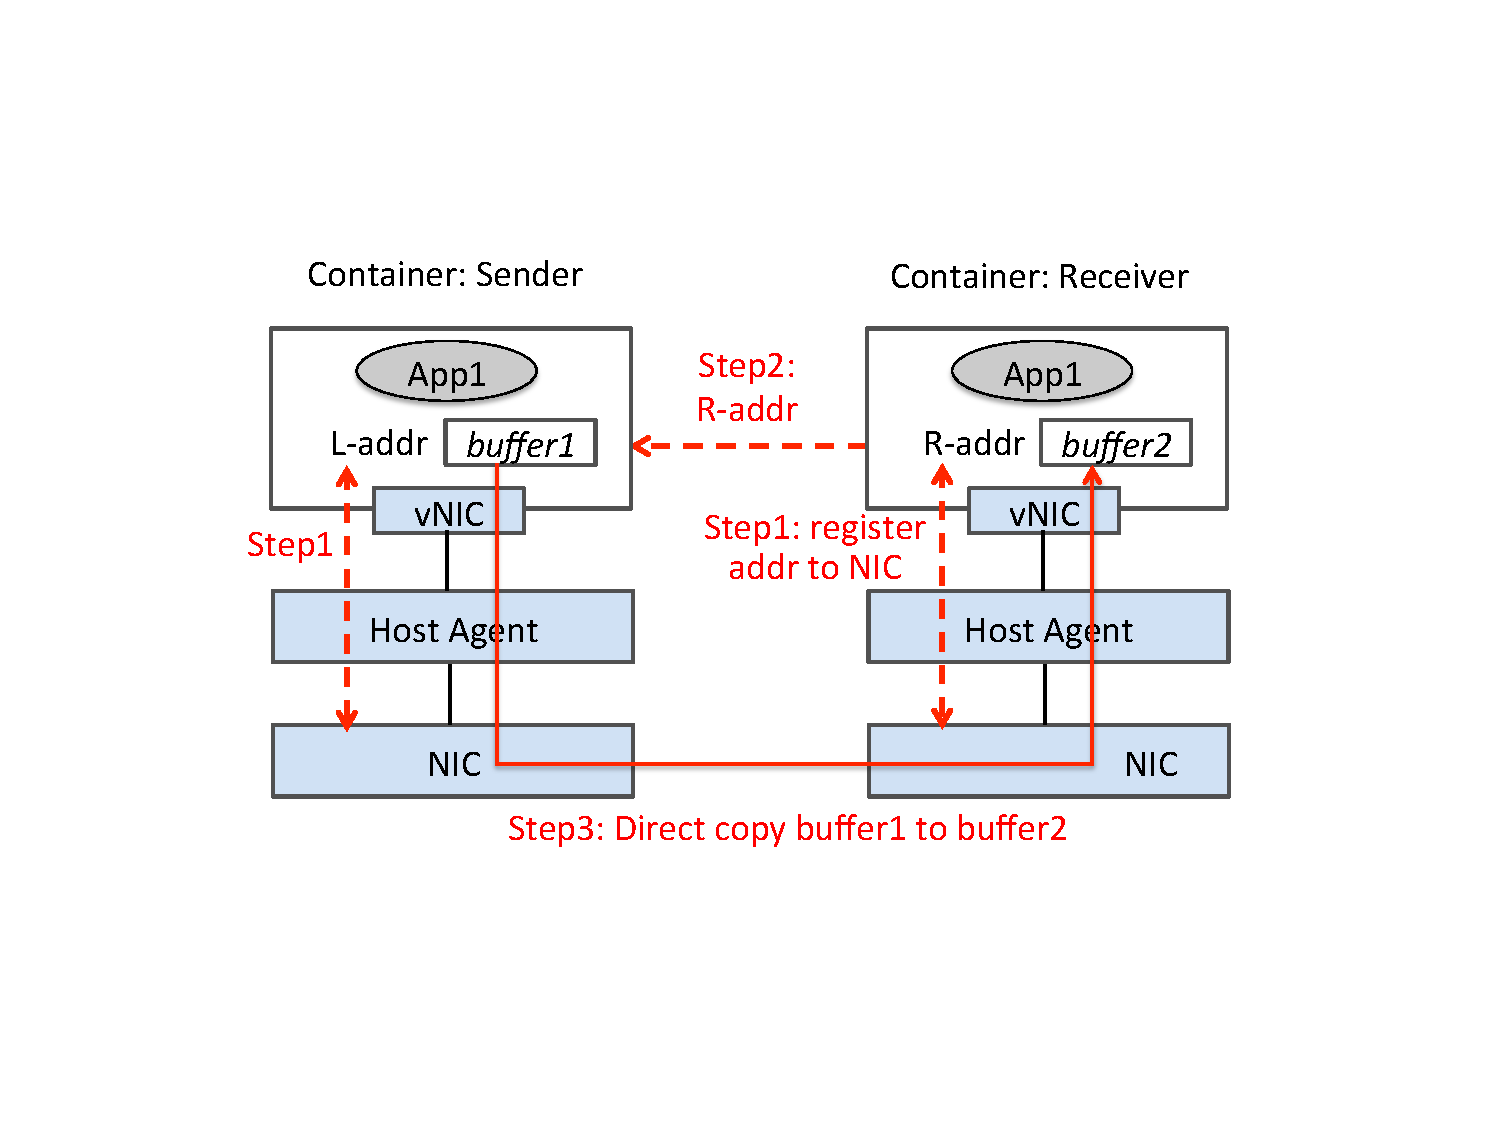
\includegraphics[width=0.45\textwidth]{figures/system/sys_rdma_rdma.pdf}      
     \label{fig:sys_rdma_rdma}
     \caption{How \sysname implemented RDMA write in inter-host setting.} 
     \end{figure}

In \sysname, both the sender and receiver containers have a virtual RDMA NIC.
In Step 1, the sender creates a shared-memory block and write data, and then 
the local network agent will get the pointer of this shared-memory block after the sender passes it to its virtual NIC; In Step 2, after receiving the IP of 
the receiver, the local network agent will check whether the receiver is on
the same host of the sender. If the answer is "Yes", the local network agent will
directly leverage the receiver's virtual NIC to notify it that a memory block 
from RDMA is ready to read with the pointer of the shared-memory block. 
Otherwise, the sender's local network agent will perform an actual RDMA write
with the receiver's local network agent, and the latter will put the received data into a shared-memory and pass it to the receiver container via its virtual NIC.
     
     \begin{figure}[ht]
     \centering 
     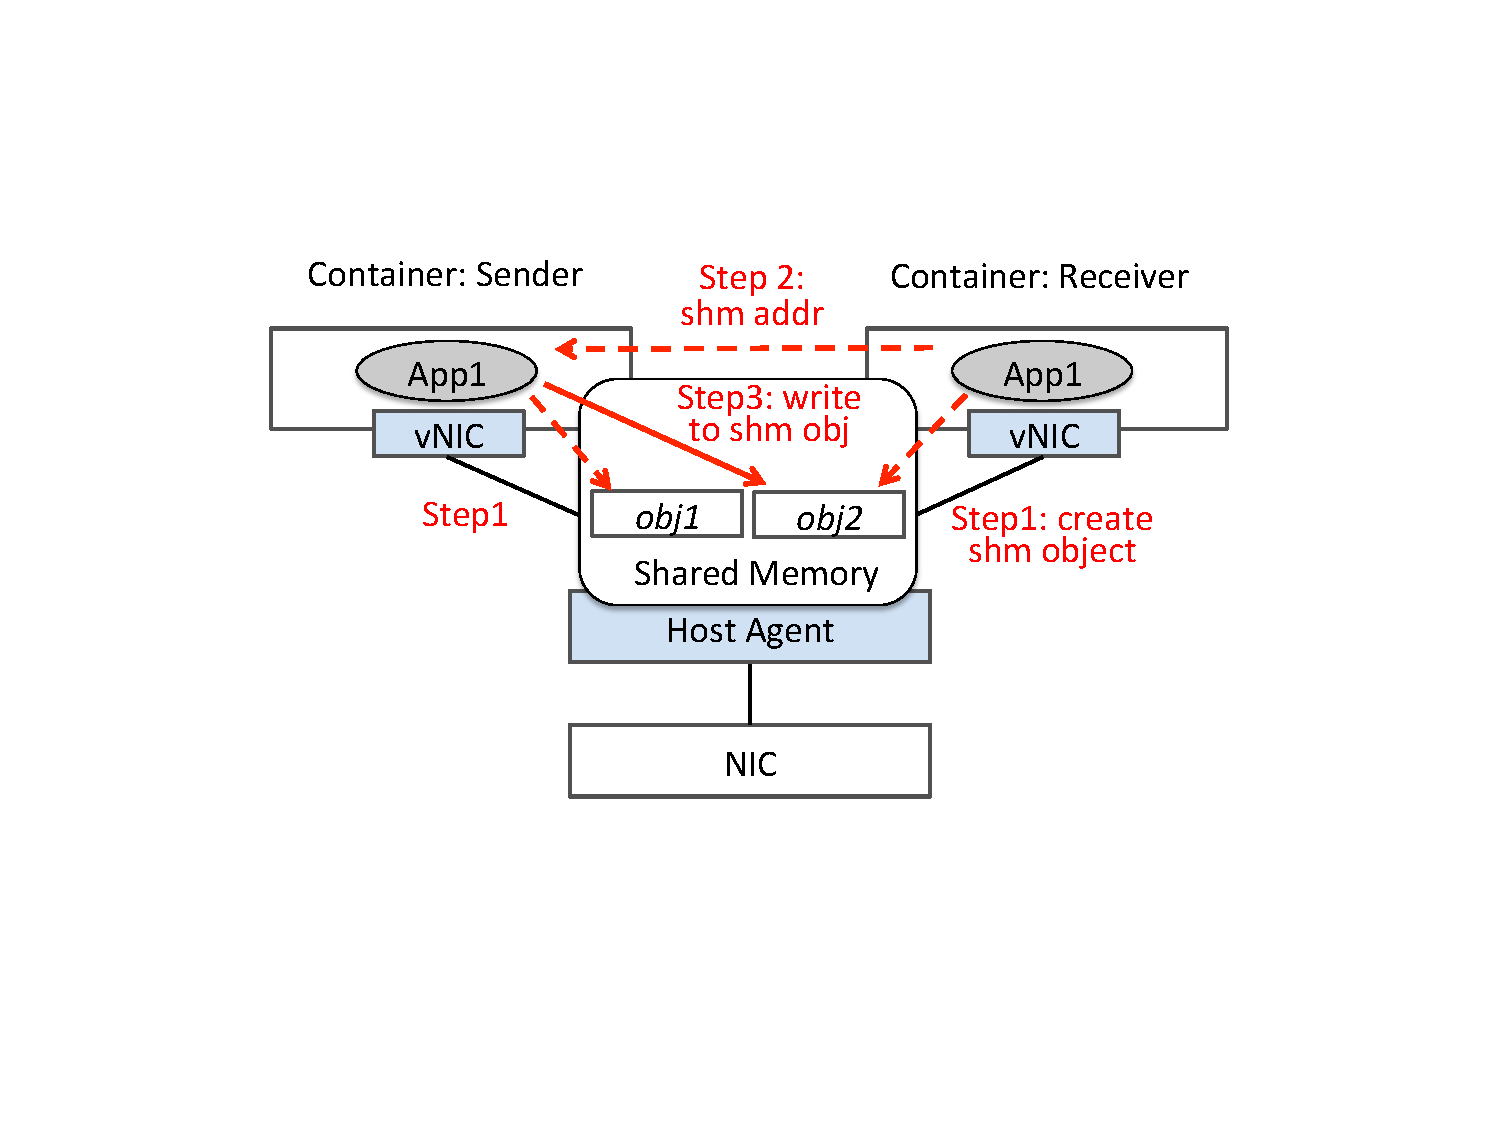
\includegraphics[width=0.45\textwidth]{figures/system/sys_rdma_shm.pdf}      
     \label{fig:sys_rdma_shm}
     \caption{How \sysname implemented RDMA write with shared memory in intra-host setting.} 
     \end{figure}
     
     \begin{figure}[ht]
     \centering 
     \begin{subfigure}
     \centering 
     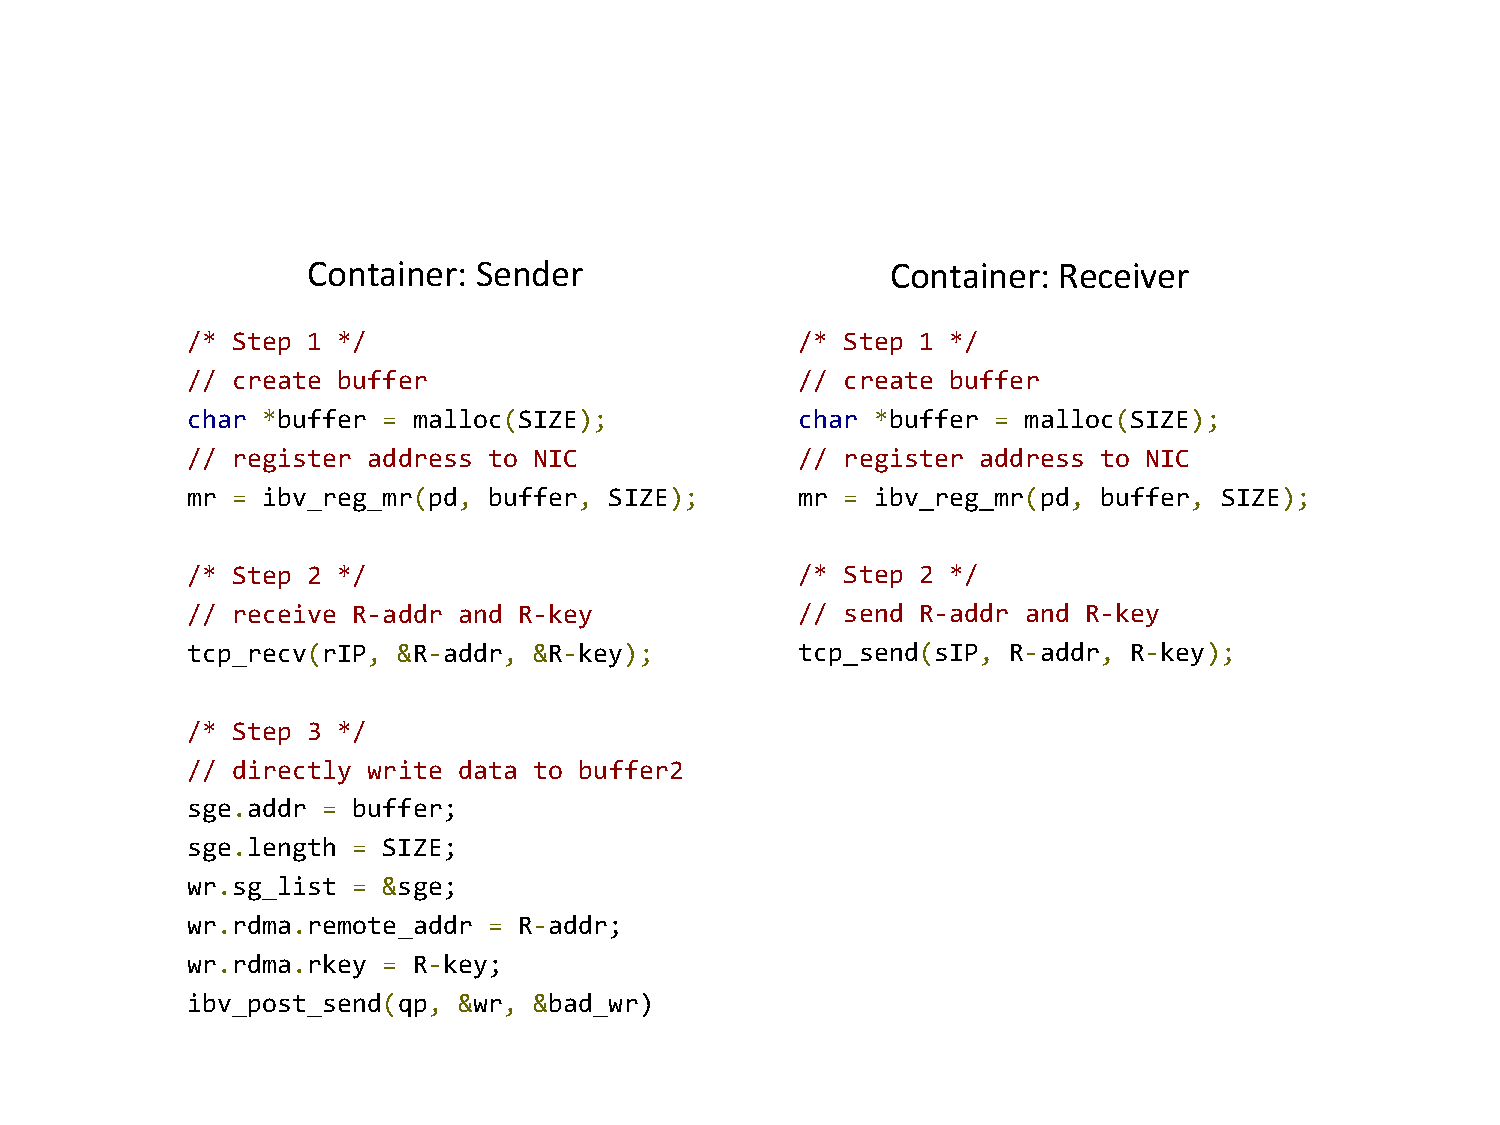
\includegraphics[width=0.45\textwidth]{figures/system/sys_rdma_code.pdf}
     %\caption{} 
     \end{subfigure}
           
     \begin{subfigure}
     \centering 
     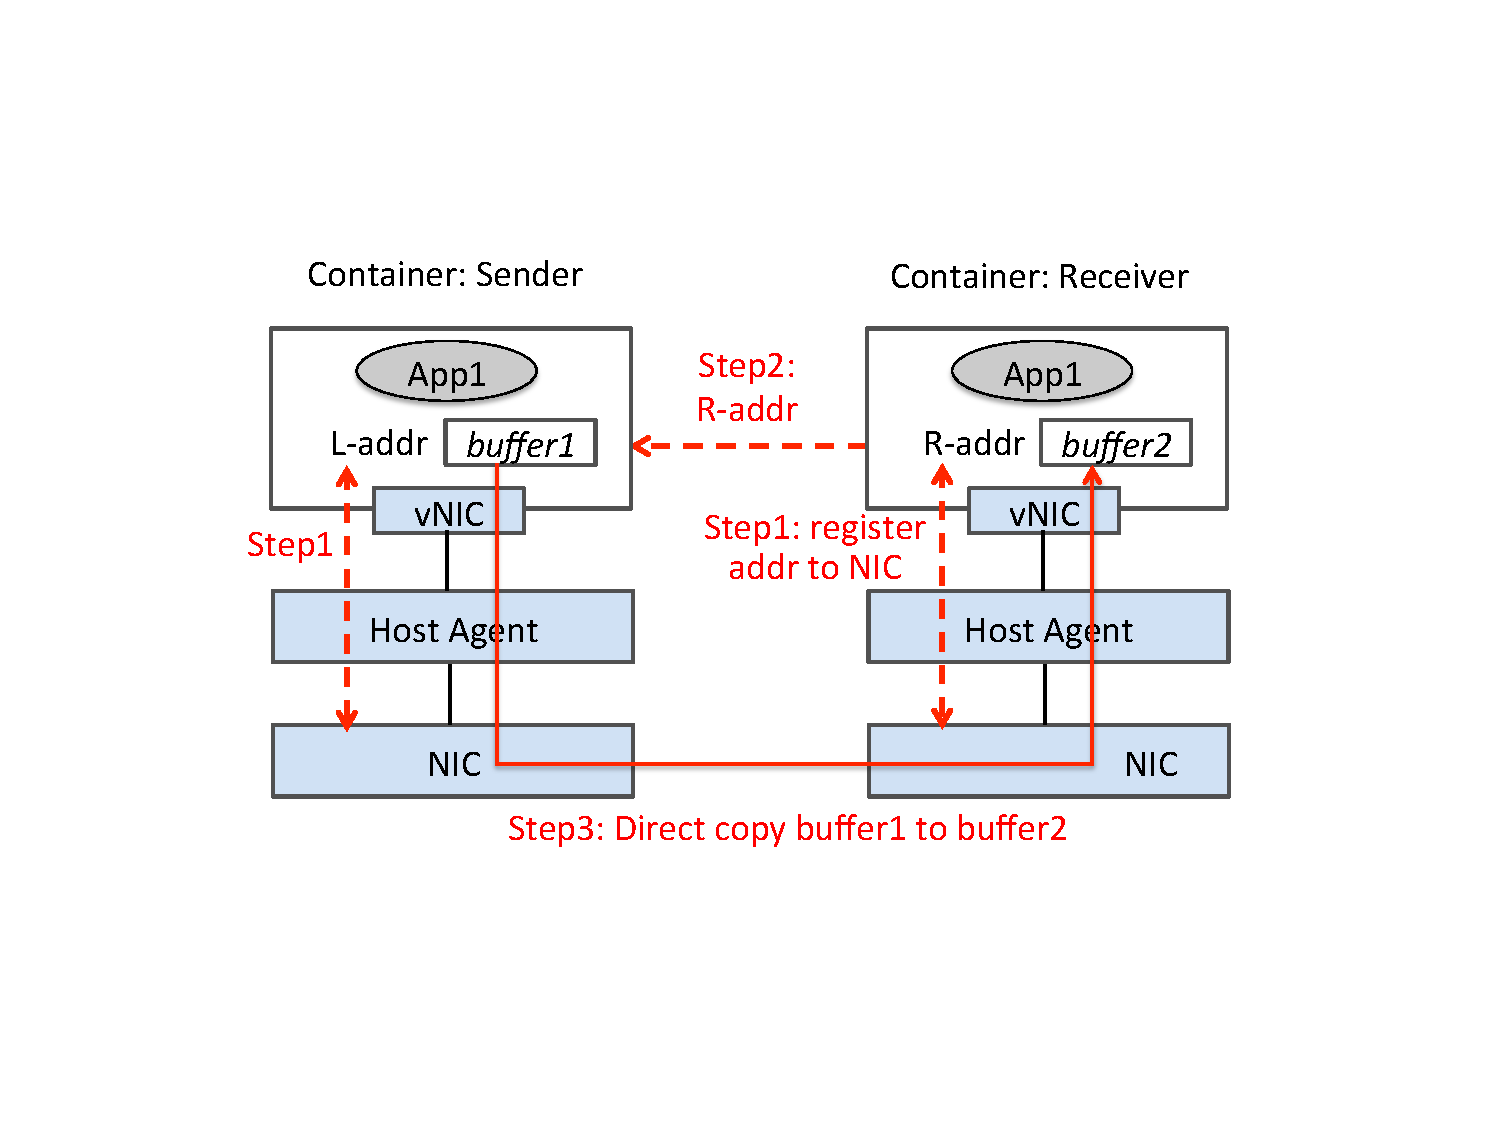
\includegraphics[width=0.45\textwidth]{figures/system/sys_rdma_rdma.pdf}      
     %\caption{} 
     \end{subfigure}
     
     \begin{subfigure}
     \centering
     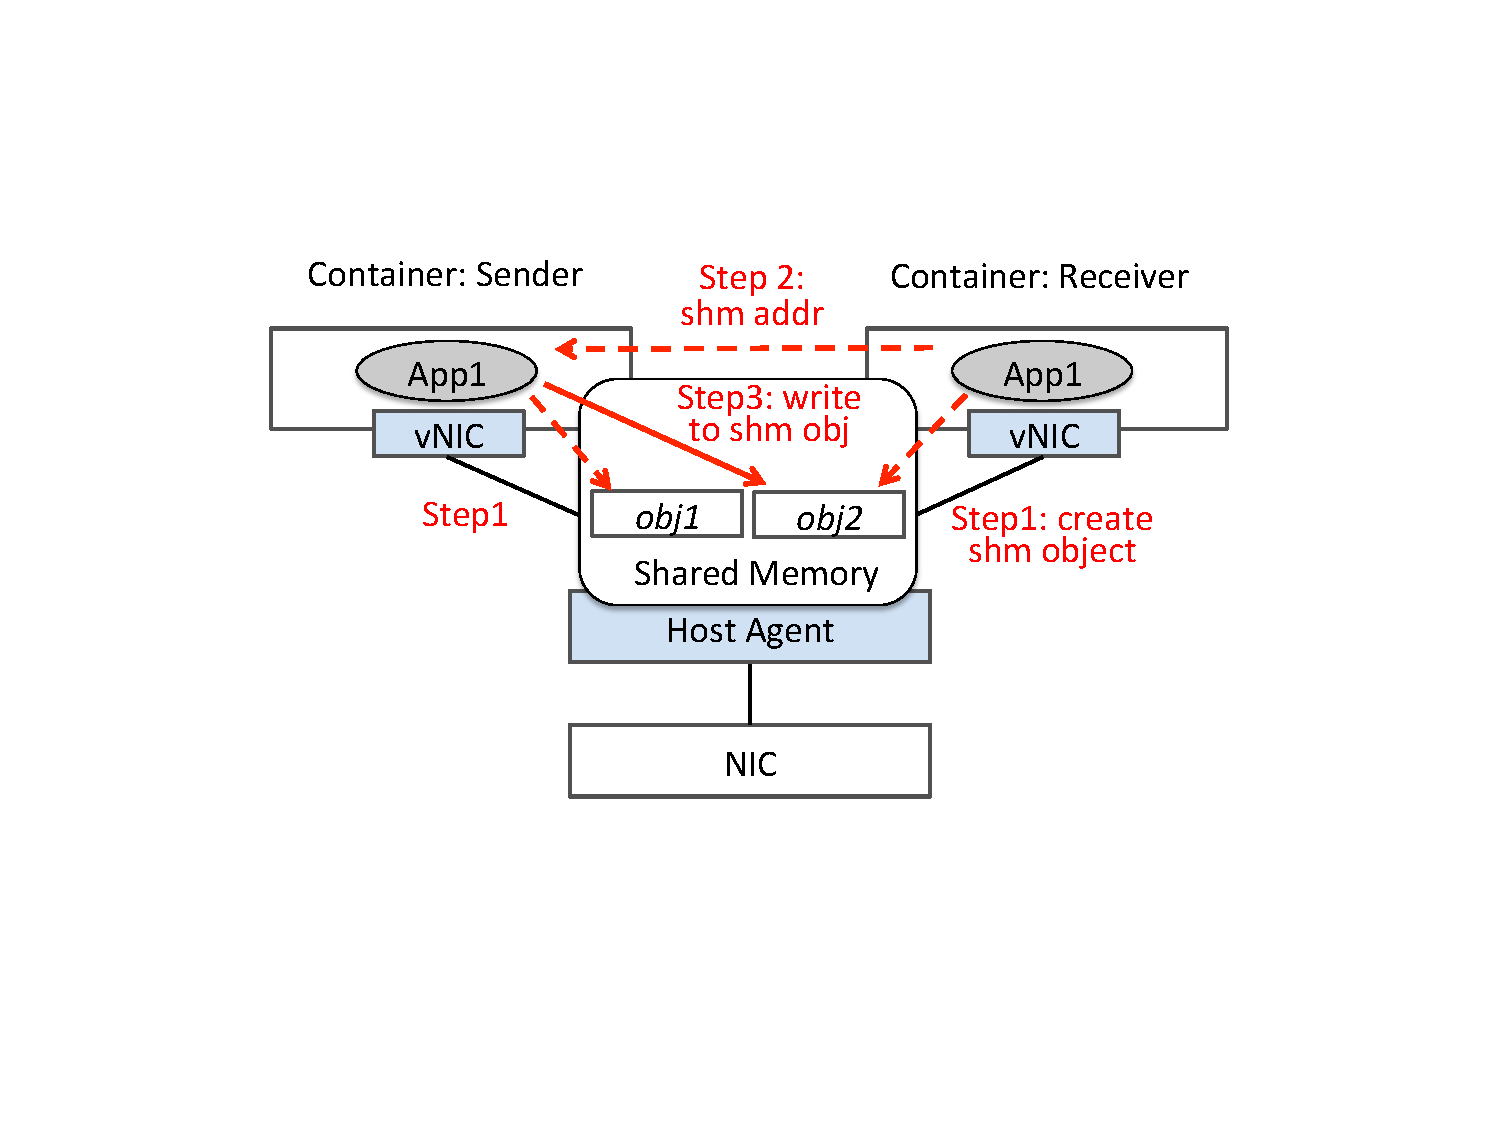
\includegraphics[width=0.45\textwidth]{figures/system/sys_rdma_shm.pdf}      
     %\caption{} 
     \end{subfigure}
     \label{fig:system_modules}
     \caption{The modules of \sysname.} 
     \end{figure}

%P1 introduce the two components we want to build
\sysname's main components includes a Orchestrator and a virtualized NIC.
The Orchestrator can figure out the most efficient way for two containers to talk with each other (e.g. 
via shared memory, rdma or dpdk) based on the location of the container or the resource
utilization of the host.
And the virtualized NIC emulates the necessary underlying resource structures 
(e.g., send queue or receive queue for RDMA). In this way, the application can
gain the desired \emph{portability}, since the application can now use the standardized  
APIs without being aware of the various underlying communication
mechanisms in different environments. 
Both of the components are shown in Figure~\ref{fig:system_modules}.

     \begin{figure}[ht]
     \centering 
     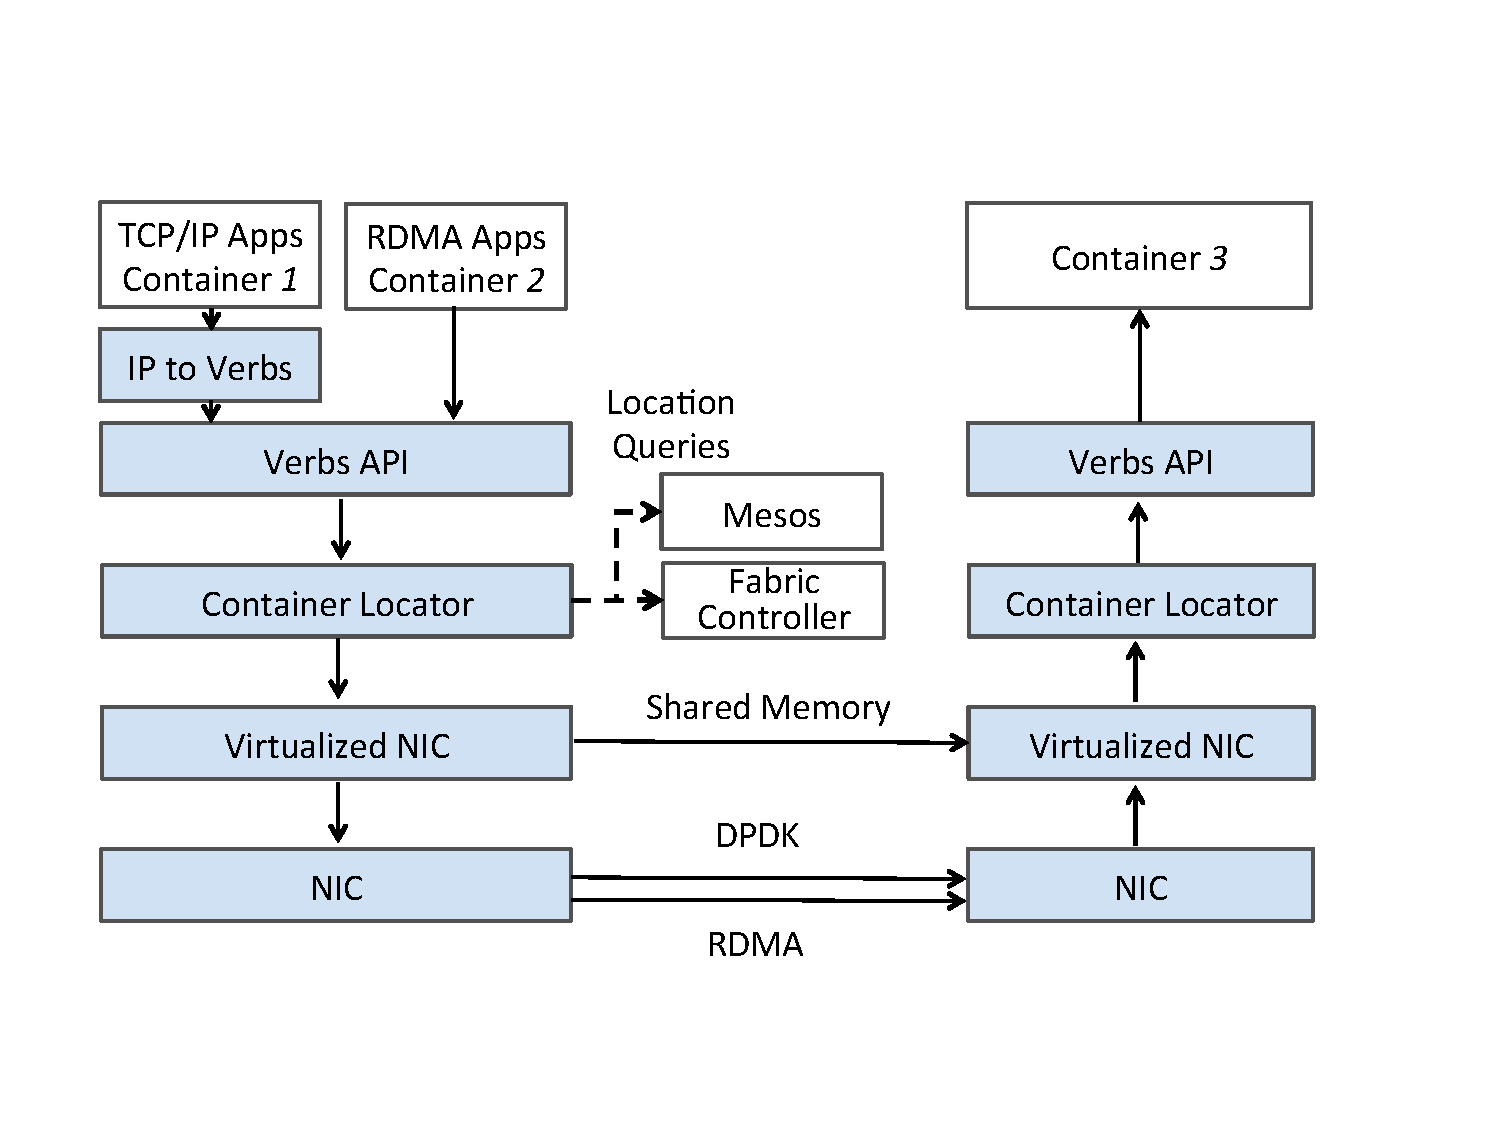
\includegraphics[width=0.45\textwidth]{figures/system/system_modules.pdf}      
     \label{fig:system_modules}
     \caption{The modules of \sysname.} 
     \end{figure}
     
      \begin{figure}[ht]
         \centering 
         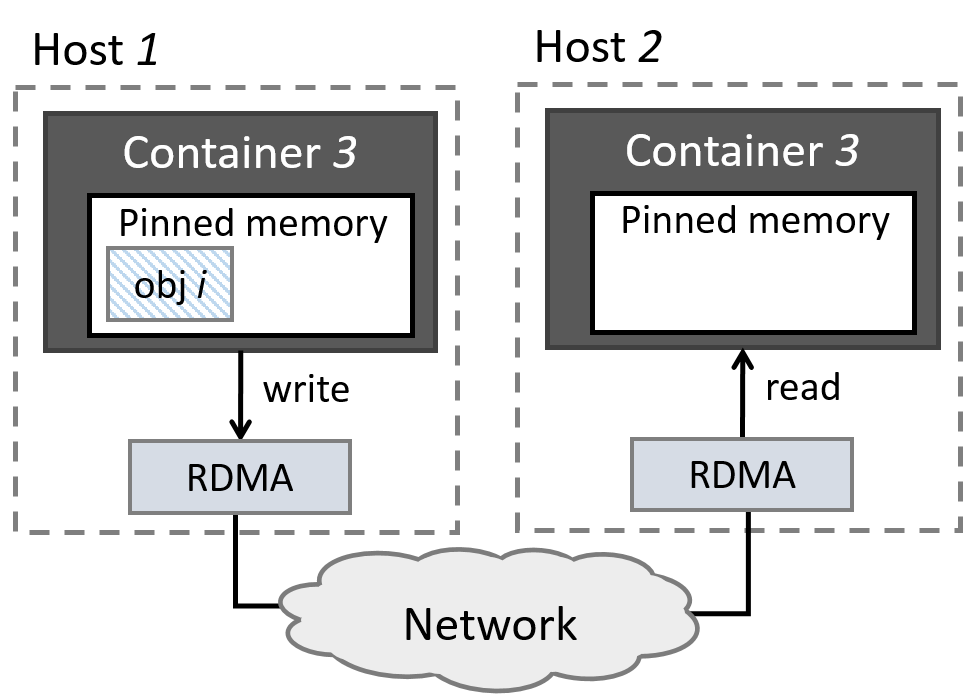
\includegraphics[width=0.2\textwidth]{figures/rdma-container.png}   
         \caption{??}   
      \end{figure}
      
      \begin{figure}[ht]
      	\centering 
      	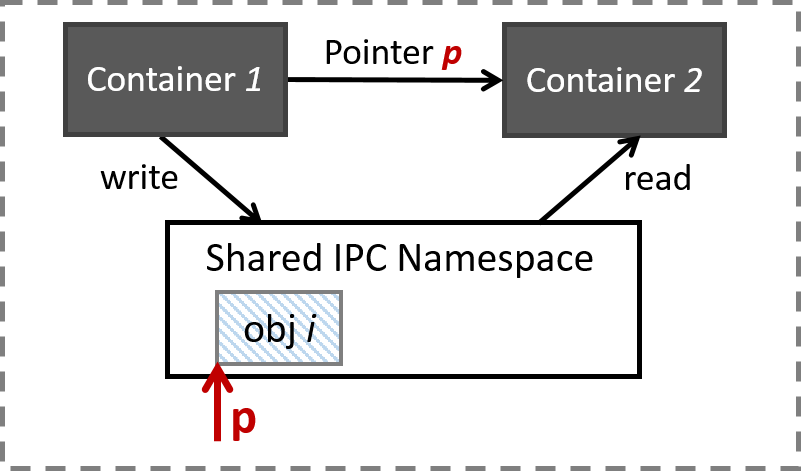
\includegraphics[width=0.2\textwidth]{figures/shared-mem-container.png}   
      	\caption{??}   
      \end{figure}

\subsection{Virtualized NIC}
The virtualized NIC (vNIC) a transparent layer between the application and the underlying network structure.
We modify the communication libraries of a container so the vNIC can intercept on the communication requests
from the applications (e.g. send request). For example, if the application is a RDMA application, we
will modify the library \texttt{libibverbs} to pass verbs calls to the vNIC.

The virtualized NIC has two roles. First, it queries the Orchestrator for the best mechanism to implement the 
communication requests, as illustrated in Figure~\ref{fig:system_modules}.
For example, if the two containers are intra-VM, it will create a shared namespace and memory objects 
for the two containers, and write the sender's data into the shared memory objects and pass the pointers of the
memory objects to the receiver container to transfer the data.

Second, the virtualized NIC (vNIC) emulates underlying network structure. 
For example, for RDMA, the vNIC will emulate the data structures including the Send Queue, 
Receive Queue, Completion Queue and Queue Pairs.
In this way, the vNIC not only maintains compatibility with currently written applications, but also
gain the desired \emph{portability}. Because the containers applications no longer need to bind to
the underlying network structure (bind to the vNIC instead), and the vNIC can be ported along with
the applications.

% as a emulation  underlying network structure
%a transparent layer between the application and the underlying network structure, dynamically choosing the best communication mechanism, while maintaining compatibility with currently written applications.

%The decision of which mechanism to chose is based on the hardware capabilities of the hosts and the physical placement of the containers, while aiming for minimal CPU overhead and high throughput. This decision and switching between communication mechanism is done completely transparent from application.

%For intra-host communication, virtualized NIC will use shared memory communication inducing minimal pressure on the CPU while reaching high throughput (~ memory bandwidth). For inter-host communication, the virtualized NIC will prioritize RDMA communication when supported by the underlying hardware. Otherwise, it will use TCP/IP communication. 


\subsection{Orchestrator}
The Orchestrator is a logic module to intelligently decide the most
efficient way to implement the communication request based on the locations
of the containers or the resources utilization of the host.

     \begin{figure}[ht]
     \centering 
     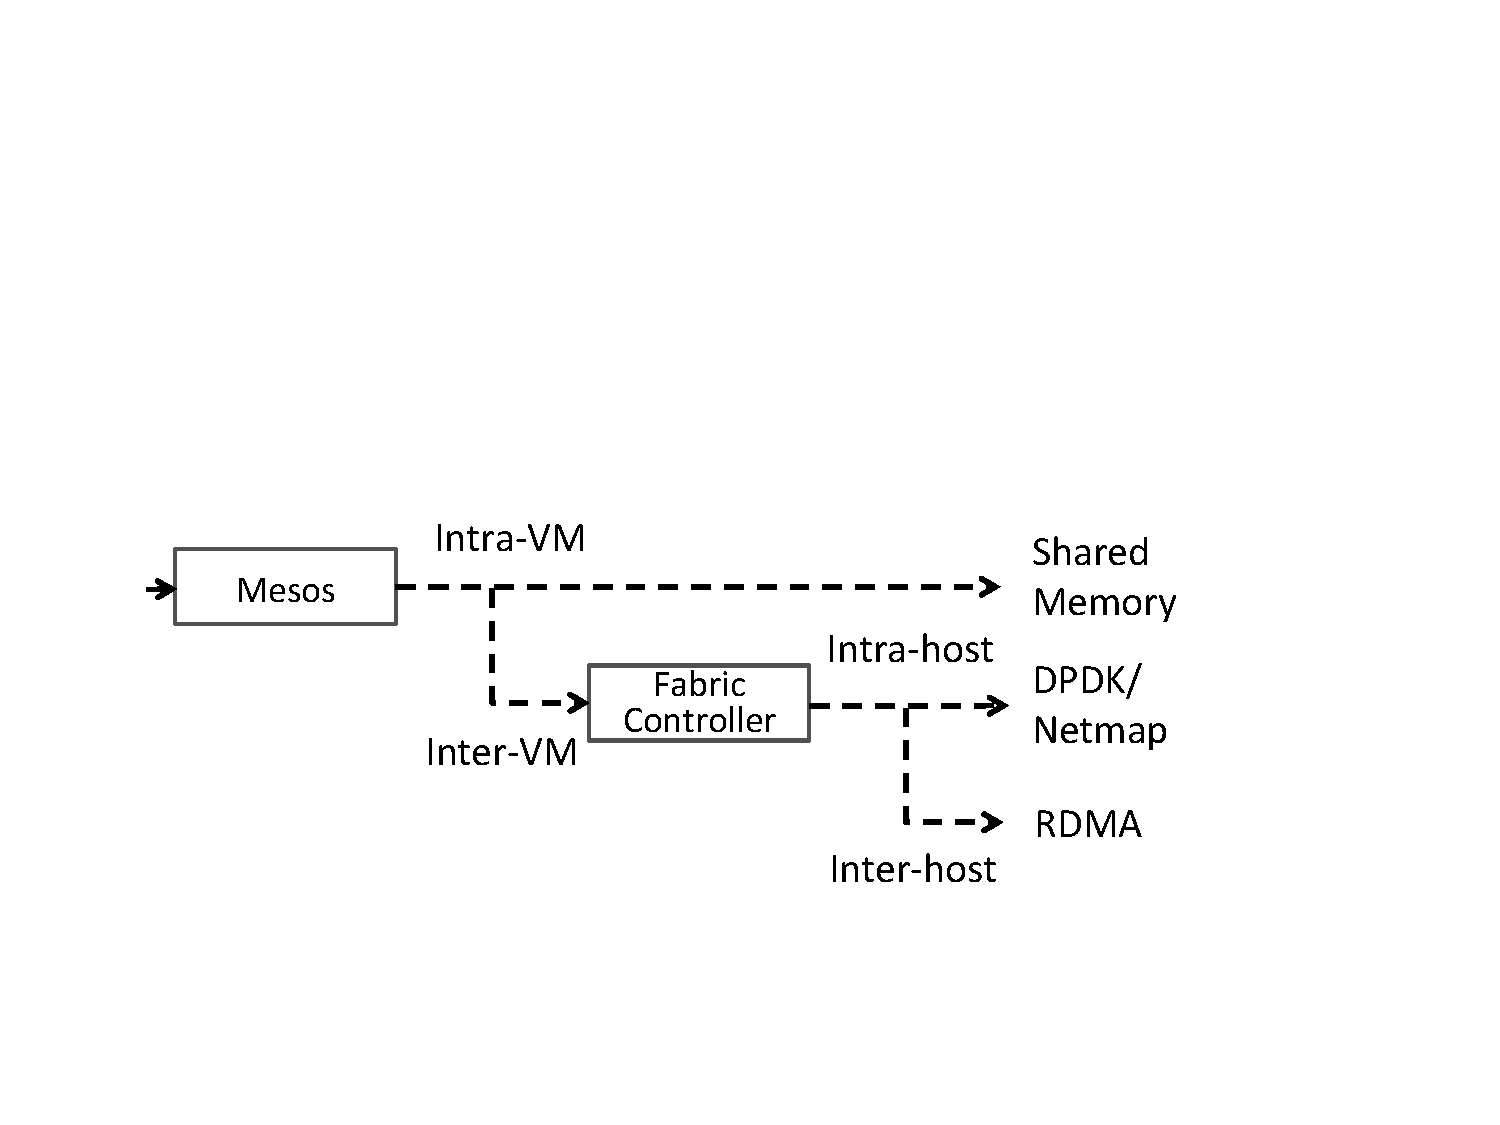
\includegraphics[width=0.45\textwidth]{figures/system/system_locator.pdf}      
     \label{fig:system_locator}
     \caption{The logic flow of Orchestrator.} 
     \end{figure}

Suppose the decision is only based on the location of the containers, the logic will be as follows.
The Orchestrator send queries to Mesos (resource manager) and the cloud's Fabric Controller to locate
the sender/receiver containers and decide the most efficient way they talk with each other.
The logic flow of this process is as shown in Figure~\ref{fig:system_locator}.
For example, given a send request, the Orchestrator will query Mesos to figure out if the 
sender/receiver containers are intra-VM or inter-VM. 
For intra-VM containers, the Orchestrator will raise a flag to notify the virtualized NIC to
send the data via shared memory.
For inter-VM containers, the Orchestrator will then quire if the two containers are intra-host
or inter-host.
If the containers are inter-VM but intra-host, Orchestrator will tell the virtualized NIC to send
the data via fast data pass across VMs in the same machine, such as NetVM\cite{} or netmaps\cite{}.
Or if the containers are inter-host, RDMA would be the most efficient way to perform the data transfer.

\tianlong{There should be some design decisions to support the above logic in design section.}

%We are going to add a logic module called Orchestrator inside the application's
%library for communication. For example, the  

\subsection{Put It Together}
Now let's put the components together and see the workflow of \sysname, as shown in Figure~\ref{fig:system_modules}.
Let's take two rdma applications (in container2 and container3) as an example.
Suppose application in container2 (app2 in short) issues a send data to container3 request via standardized Verbs API.
The vNIC will intercept the request and query the Orchestrator. 
Then the orchestrator will query Mesos or Fabric Controller to obtain the locations of 
container2 and container3. Then Orchestrator will send a decision of the best mechanism to the vNIC.
The request will call to the emulated data structures in the vNIC (e.g. QP, SQ, RQ, CQ). And the vNIC will choose the
best mechanism (e.g. RDMA, shared memory, dpdk/netmap) to implement the request. For example, if the containers
are inter-host, RDMA will be selected. If the best mechanism is not available (e.g. NIC lack of RDMA support), it will
fall back to the sub-optimal mechanism (e.g., TCP/IP).

\fi
